\documentclass[10pt,a4paper]{article}
\usepackage{homework} % See homework.sty %
\usepackage{graphicx}
\usepackage{float}
\usepackage{array}
\usepackage[export]{adjustbox}  
\newcolumntype{M}[1]{>{\centering\arraybackslash}m{#1}}

\author{1155193237 - Yu Ching Hei\\email: chyu2@cse.cuhk.edu.hk}
\title{CENG3420 - Computer Organization \& Design\\Lab1 Report}
\pagestyle{fancy}
\renewcommand{\headrulewidth}{0pt}
\fancyhf{}
\cfoot{\thepage}
\date{Date: \today}
\begin{document}
\maketitle

\question{
	\label{Question1}
    Write a RISC-V assembly program step by step as shown below:
    \begin{enumerate}
        \item Define three variables var1, var2 and var3 which will be loaded from terminal using syscall.
        \item Increase var1 by 3, multiply var2 by 2.
        \item increase var3 by var1 + var2.
        \item print var1, var2 and var3 to terminal using syscall.
    \end{enumerate}
}

\begin{ans} 

    First, I declared a variable of datatype “.ascii” and named it as endl, which stored the constant 
string literal `\textbackslash n'. 

    Then the program will require the user to input 3 integers by loading immediate 5 to change the system call 
mode into readInt mode. Then issue a system call to request for input. After the system call, the integer would 
be stored at a0 as return value. Then I perform the data copy from a0 to t0 by mv a0, t0 and the same for t1 
and t2 as well. Then I perform the arithmetic to the data. By running addi t0, t0, 3, I can add a hard code 
constant 3 to t0, then store back to t0 (t0 = t0 + 3). 
 
    Since mul instruction does not accept immediate, so I loaded a register t3 with the multiplier “2” using the li t3, 2. 
 
    Then I perform the multiplication by multiplying t1 with t3 and then stored back to t3 (t1 = t1 * t3) by doing mul t1, t1, t3. 
Followed by the last modification to the numbers, since we cannot sum a value with 2 other value at the same time, to perform 
var3 = var3 + var1 + var2, I have to do the addition twice. 
 
	First I added t0 to t2 then stored it back to t2, then I add another t1 to t2 and then store it back to t2. For a cleaner code, 
I wrote a function for printing prtNL for printing a new line character after printing each variable. 
 
	In the prtNL function, I first changed the mode of system call to 4 which is printString from address. 
Then I load the address from memory by la a0, endl. Then I issue a system call and return to the return address. 
 
	Now I start to print the variable to the console one by one. I change the system call mode to 1 which is printInt, 
then copy the data from the registers that store the data representing var1, var2 and var3 respectively 
to the a0 register which is the function argument register. 
 
	Finally, I loaded register a7 with 10, which changes the system call mode to exit the program with code 0. 
 
\break

\begin{table}[htbp]
    \begin{center}
        \caption{Main Code for Question 1}
        \begin{tabular}{|M{2.5cm}|M{3.5cm}|M{2cm}|M{4cm}|}
            \hline
            Input Integer & Add and Multiply & Print Integer \& Exit & New Line Function\\
            \hline
            \centering
            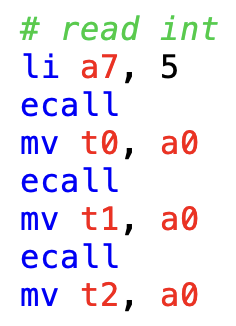
\includegraphics[scale = 0.5]{Lab1-1-1.png} &
            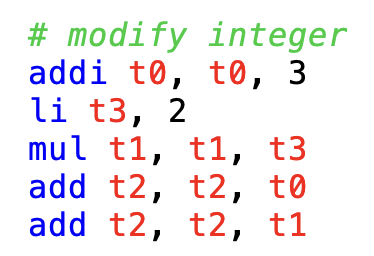
\includegraphics[scale = 0.5]{Lab1-1-2.png} &
            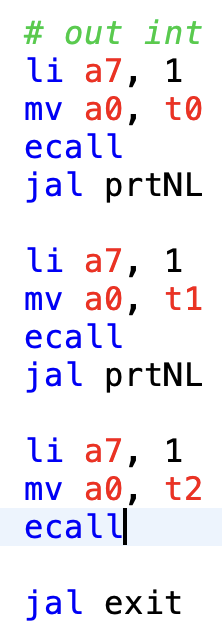
\includegraphics[scale = 0.5]{Lab1-1-3.png} &
            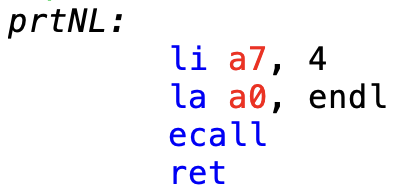
\includegraphics[scale = 0.5]{Lab1-1-4.png} \\
        \hline
    \end{tabular}
    \end{center}
\end{table}

\begin{figure}[H]
    \caption{Console Results}
    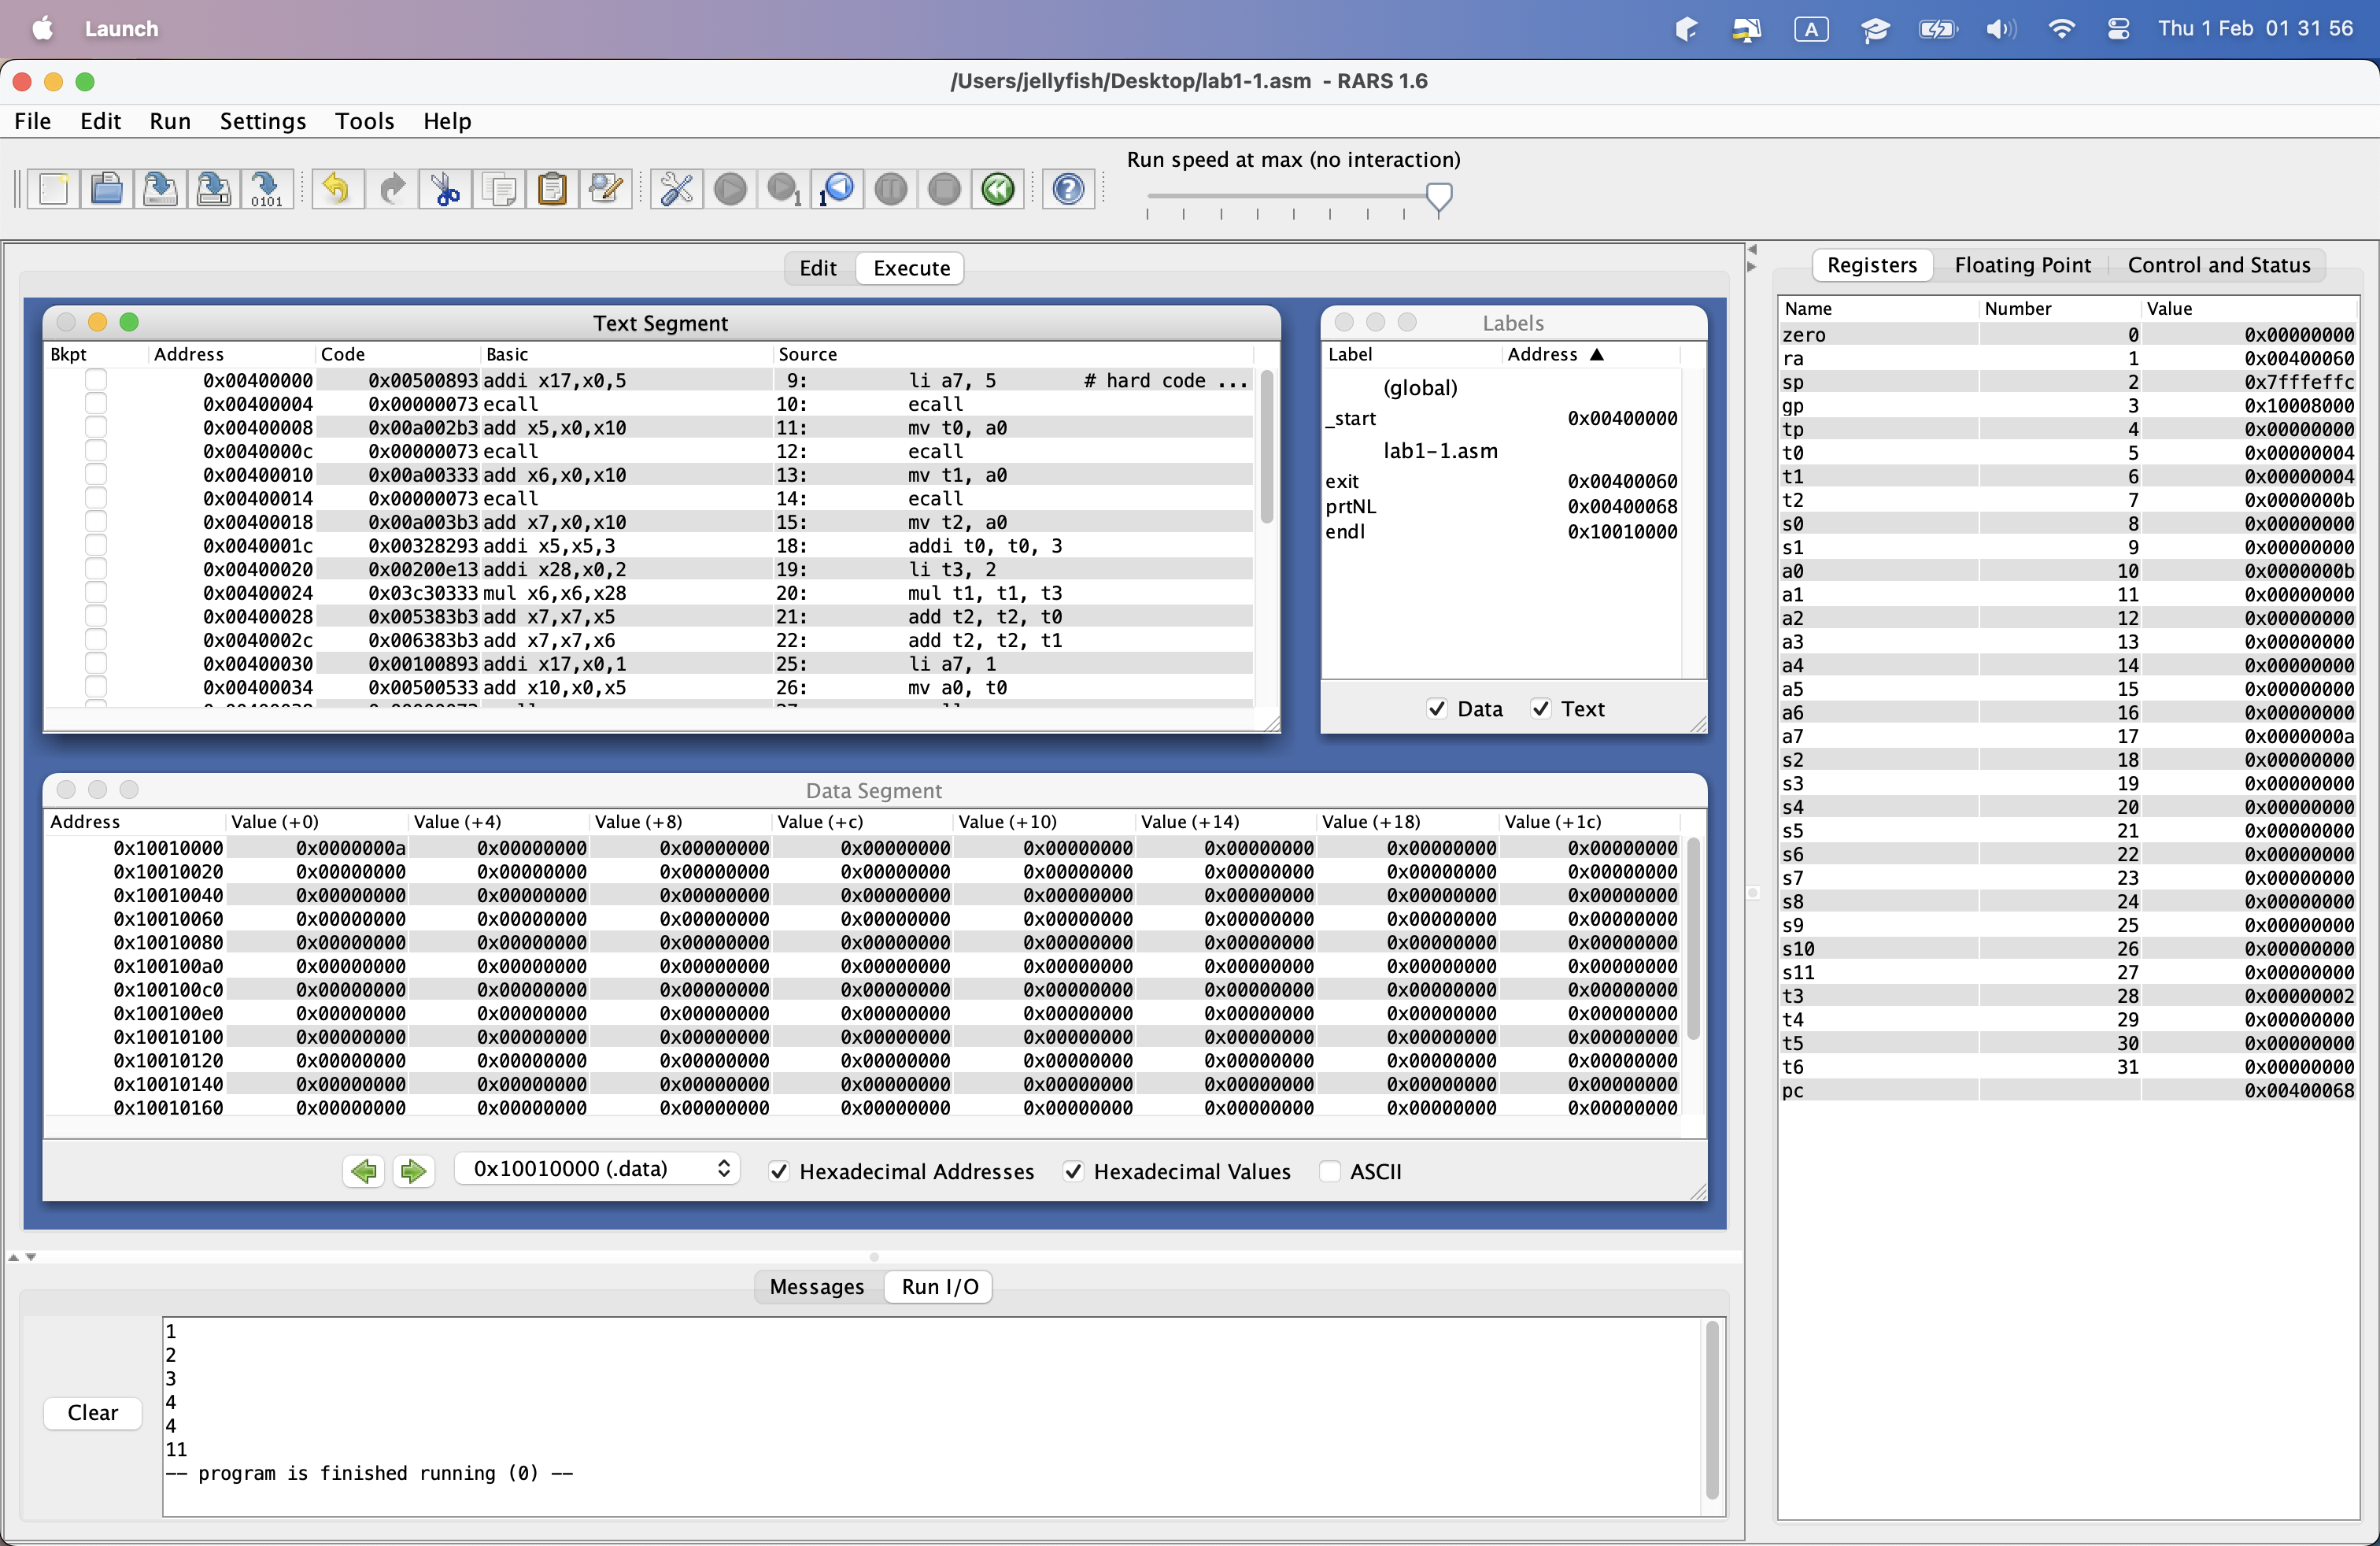
\includegraphics[width=1\linewidth]{Lab1-1-5.png}
\end{figure}
 
\end{ans}

\pagebreak

\question{
An array array1 contains the sequence -1 22 8 35 5 4 11 2 1 78, each element of which is .word. Rearrange the element order in this array such that,
    \begin{itemize}
        \item All the elements smaller than the 3rd element (i.e. 8) are on the left of it
        \item All the elements bigger than the 3rd element (i.e. 8) are on the right of it
    \end{itemize}
}
\begin{ans}

    \noindent Fisrt I have created a two variables in the memory, namely: 

	\begin{itemize}
		\item array1: a .word array that contains 10 elements given in the question
		\item space: a .ascii variable that store the delimiter character ` ' for printing
	\end{itemize}
	8 is the pivot, -1, 5, 4, 2, 1 are the element smaller than 8 in the array, and we have 22,
	35, 11, 78 larger than 8. Detail are shown in the following parts. 
	\begin{enumerate}
		\item I swapped the pivot(8) with the final element in the array
		\item Then I call the PARTITION function to do the partition by passing in 3 parameter to the function
		 	namely array address(s0), lowest index(s1), highest index(s2)
		\item In the PARTITION function, it takes in 3 parameter, they are s0(Array1 location), s1(permanent storage of lowest position) and s2(permanent storage of the highest position). It scans for any element that is smaller than the pivot, then swap with first element that is greater than the pivot
		\item After finished one round of searching and swapping, the loop end and swap the pivot with the first element that is larger than the pivot
		\item Print the partitioned array
		\item Exit the program with exit code 0
	\end{enumerate}
	
    \begin{table}[htbp]
        \begin{center}
			\caption{Main Code for Question 2}
				\begin{tabular}[H]{|M{3cm}|M{12cm}|}
					\hline
					Function & Code\\

					\hline
					PARTITION function 
					& 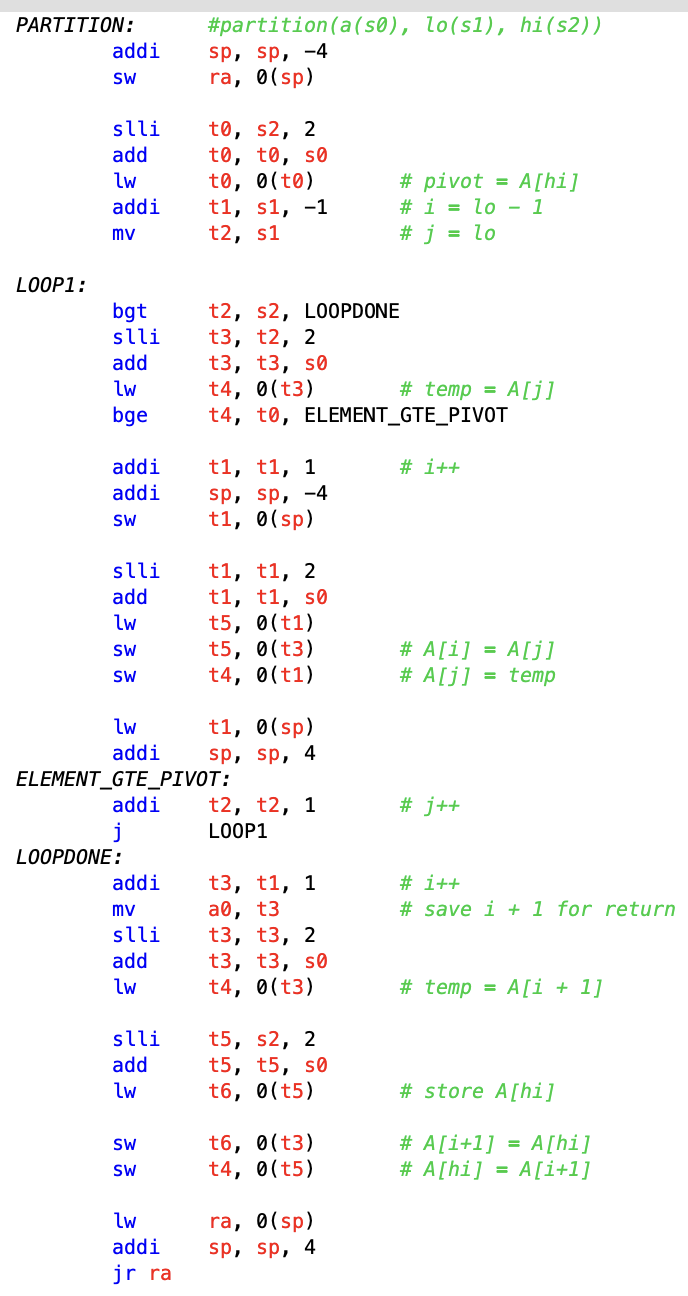
\includegraphics[scale = 0.7]{Lab1-2-2.png}\\

					\hline
					printLoop (A looping function to store the elements in the temp array into the original array and print them out one by one)
					& 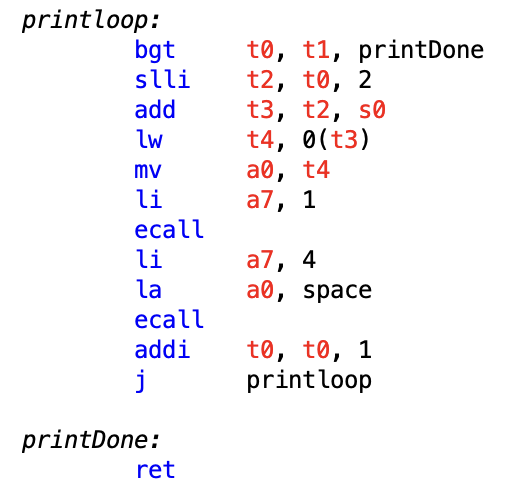
\includegraphics[scale = 0.7]{Lab1-2-3.png}\\
					\hline
				\end{tabular}
		\end{center}
        
    \end{table}
    \break
	\begin{figure}[H]
		\caption{Console Results}
		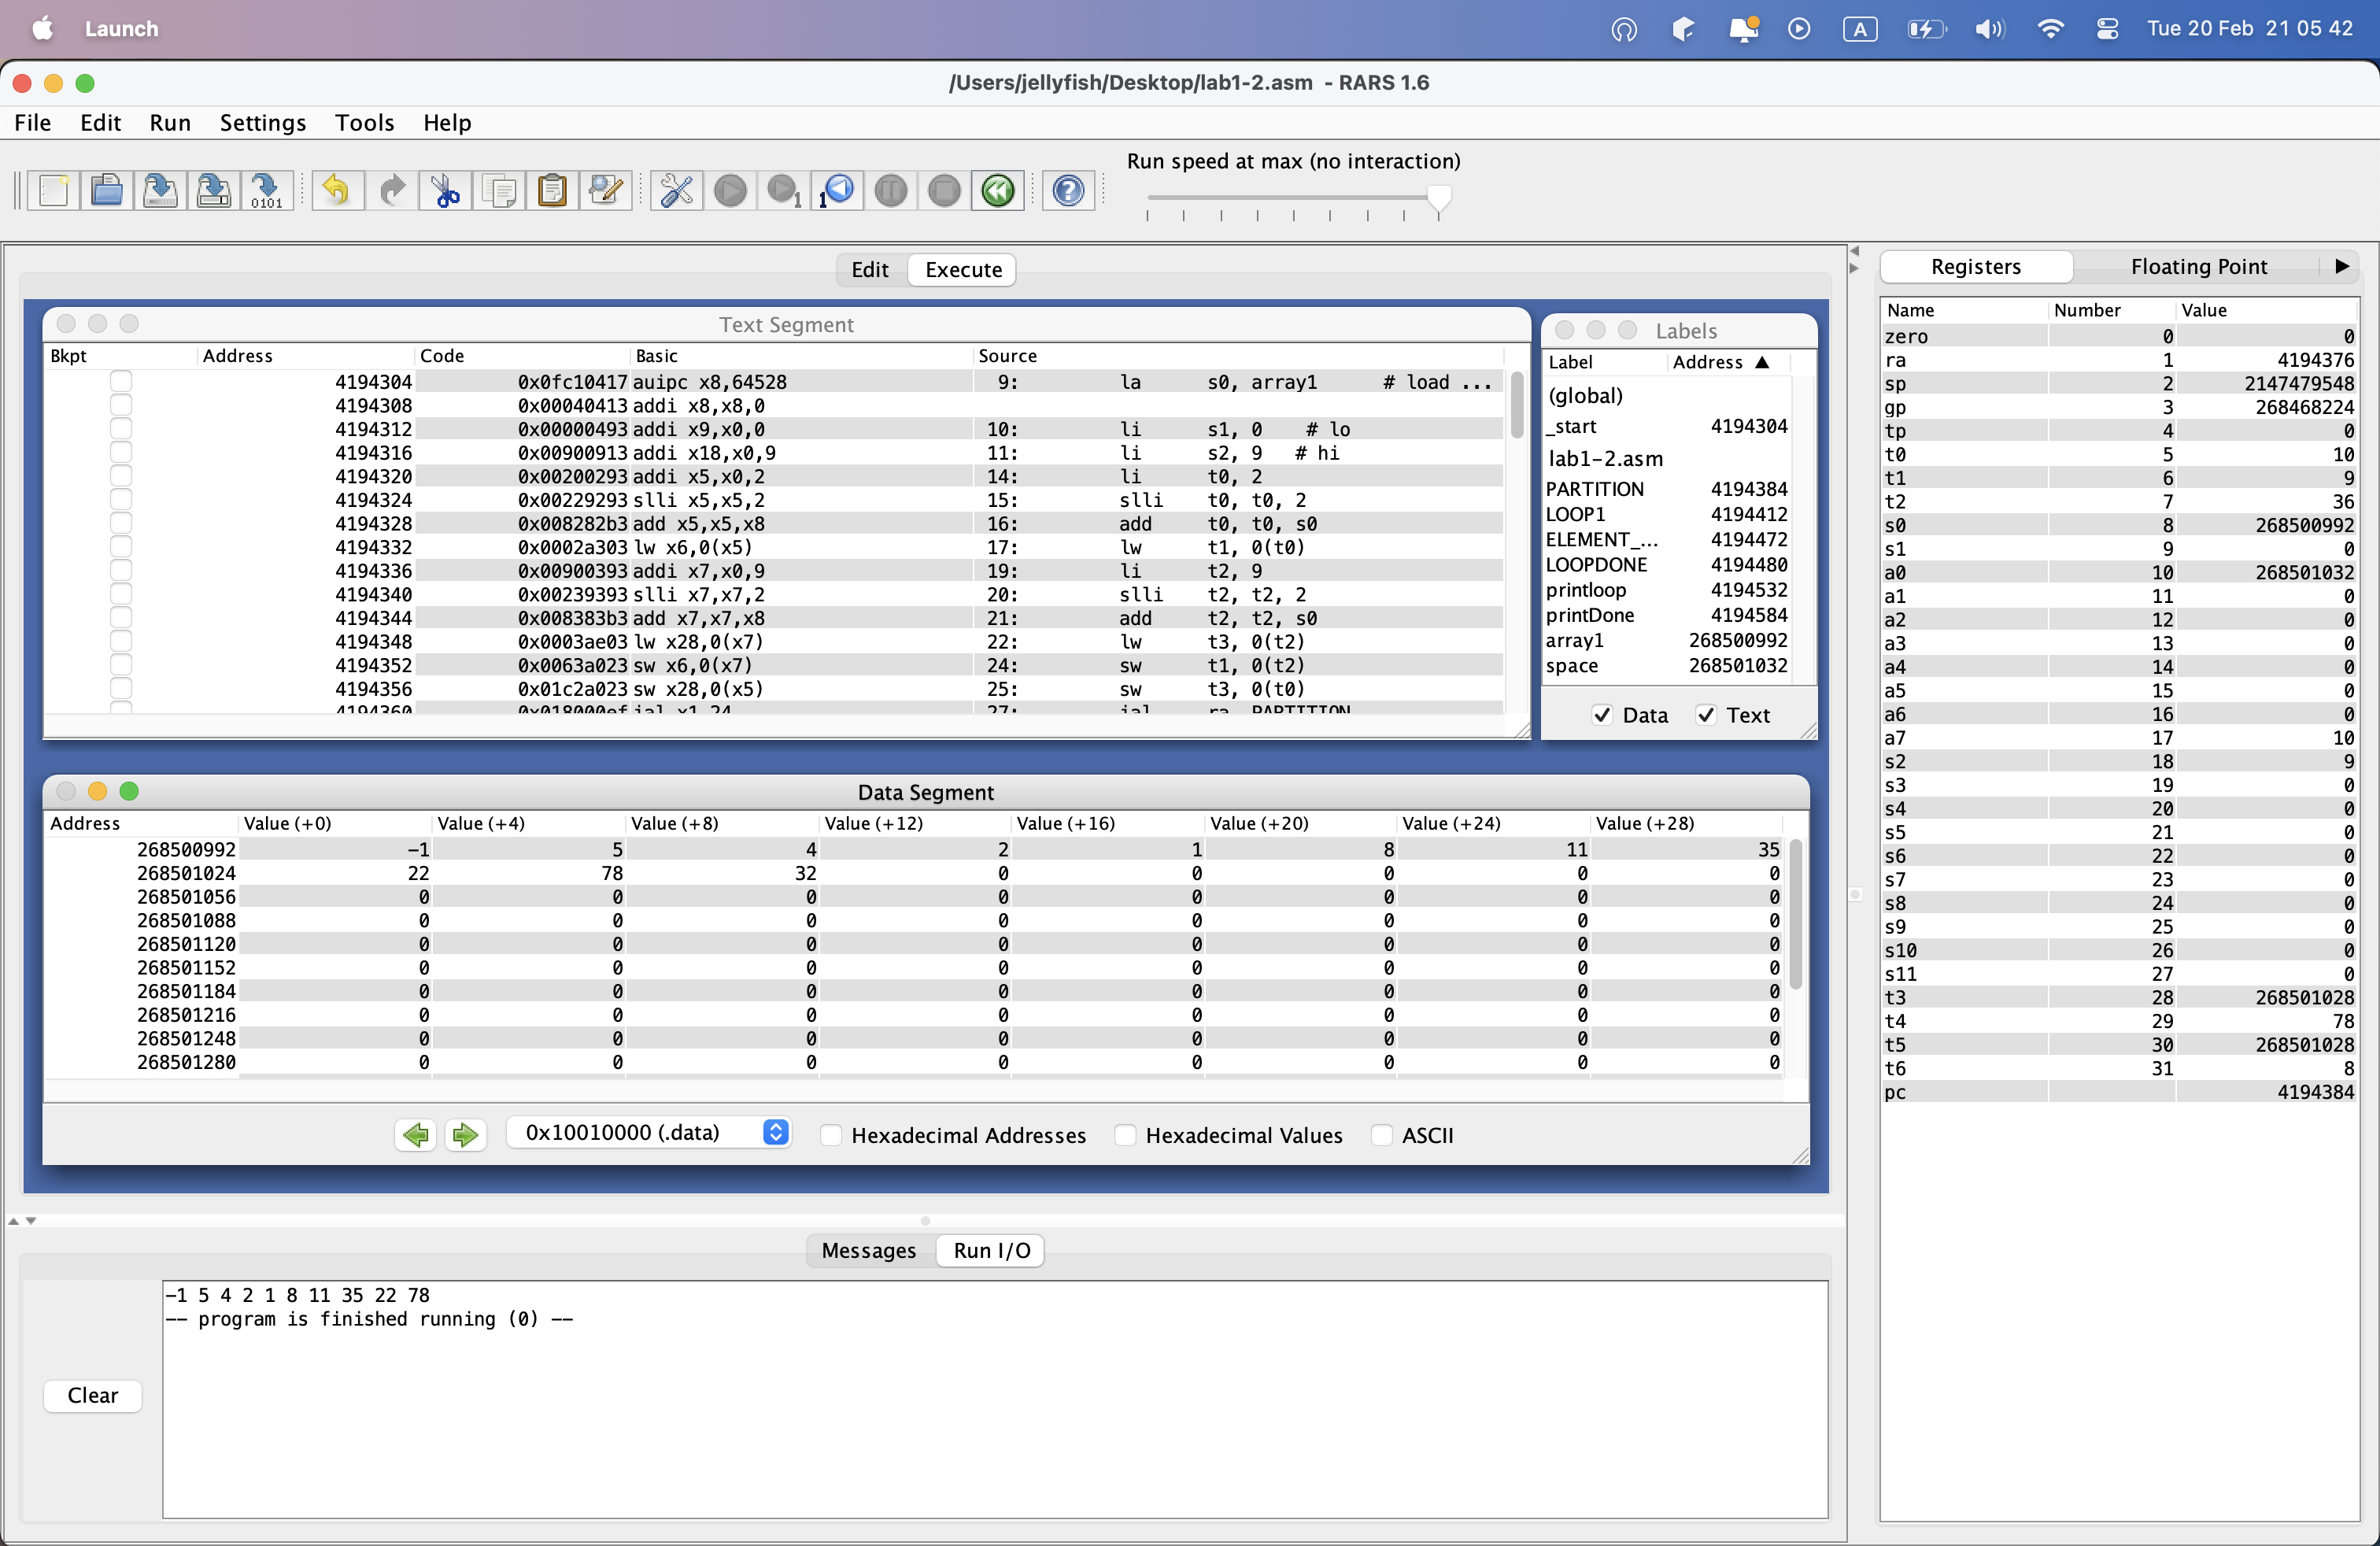
\includegraphics[width=1\linewidth]{Lab1-2-1.png}
	\end{figure}
    
\end{ans}

\pagebreak

\question{
    Implement Quicksort $w.r.t.$ the following array in ascending order with RISC-V
    assembly programming:
    
    In the first line, you will be given an integer n (2 $<$ n $<$ 100), representing the
    array size. In the second line, a sequence of n integers will be provided.
}
\begin{ans}

	\noindent In this question, I have created 2 variables in memory, namely:
	\begin{itemize}
		\item array: a .word array for storing the integer input and sorting
		\item space: a .ascii variable that store the delimiter character ` ' for printing
	\end{itemize}
	\noindent I solve this question with the follwoing stpes: 
	\begin{enumerate}
		\item For the input part, the first input will be the number of array elements, let's call it n. (n - 1) is the index of the last element of the array, at the same time it could also be used as a looping bound for both input and output. 
		\item For input and output, I have used the same looping structure, but by passing in a0 = -1 (a0 < 0) and a0 = 0, the function of the loop will be changed to input and output respectively since I have set a0 as a parameter and determine whether it should branch to input action or output action. 
			This could help reduce the redundancy of similar code and simplify the code. 
		\item For the quicksort part, I have done the typical way of quicksort which is basically if (low $<$ high) then do the partition and then do the quicksort for the left and right part of the pivot respectively. It takes in 3 parameters, namely s0(array location), a1(low w.r.t each partition), a2(hi w.r.t each partition), 
			they are further passed into the PARTITION function under the quicksort function. 
		\item I have reused the same PARTITION function as done in Lab1-2, but in this question, I have changed the parameter from s0(array location), s1(permanent storage of low), s2(permanent storage of hi) into s0(array location), a1(low w.r.t each partition), a2(hi w.r.t each partition). 
		The main difference here is that in question 2, since we are not going to do multiple times of partitioning, so it is good enough to just use the low and high position of the whole array. But for quicksort, each recursion will have a new partition action. If I still use s1(lo) and s2(hi) as the parameter, there would be no changes. 
		Therefore, I have change the lo and hi to be a1 and a2, which are changed depends on the subarray that the quicksort is currently processing. It is not necessary to change s0 as well since s0 is just for the address of the array and it is never changed in each recursive call of quicksort. 
		It scans for any element that is smaller than the pivot, then swap with first element that is greater than the pivot, finally swap the pivot with the first element that is larger than the pivot. 
		\item 	After recursive call of quicksort functions, the array got partitioned into 10 subarrays that are of length of 1 element and they are sorted since the smaller element will go to the left side of the pivot. 
		\item 	Finally, print the sorted array separated by `` '' and exit the program with exit code 0. 
	\end{enumerate}
	*The console input is separated by `\textbackslash n' while the output is the final line separated by ` ' character. 
	
	\begin{table}[htbp]
        \begin{center}
			\caption{Main Code for Question 3}
				\begin{tabular}[H]{|M{3cm}|M{12cm}|}
					\hline
					Function & Code\\

					\hline
					Loop handeling input and output
					& 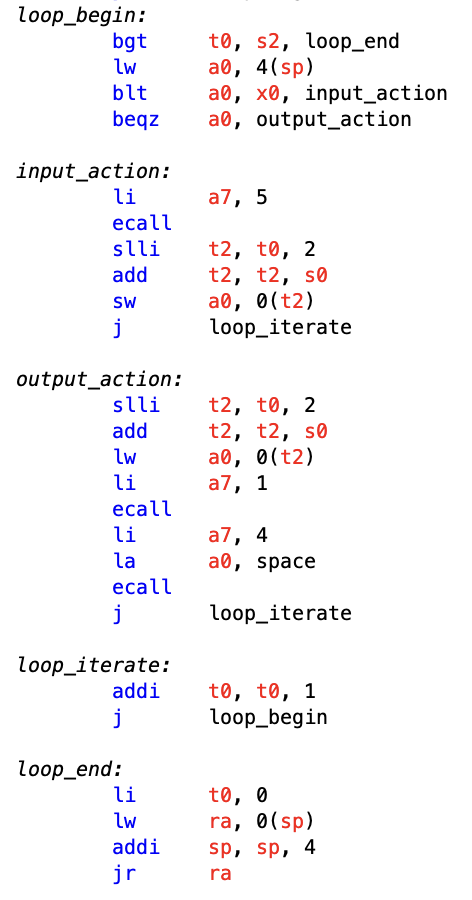
\includegraphics[scale = 0.7]{Lab1-3-2.png}\\

					\hline
					QUICKSORT
					& 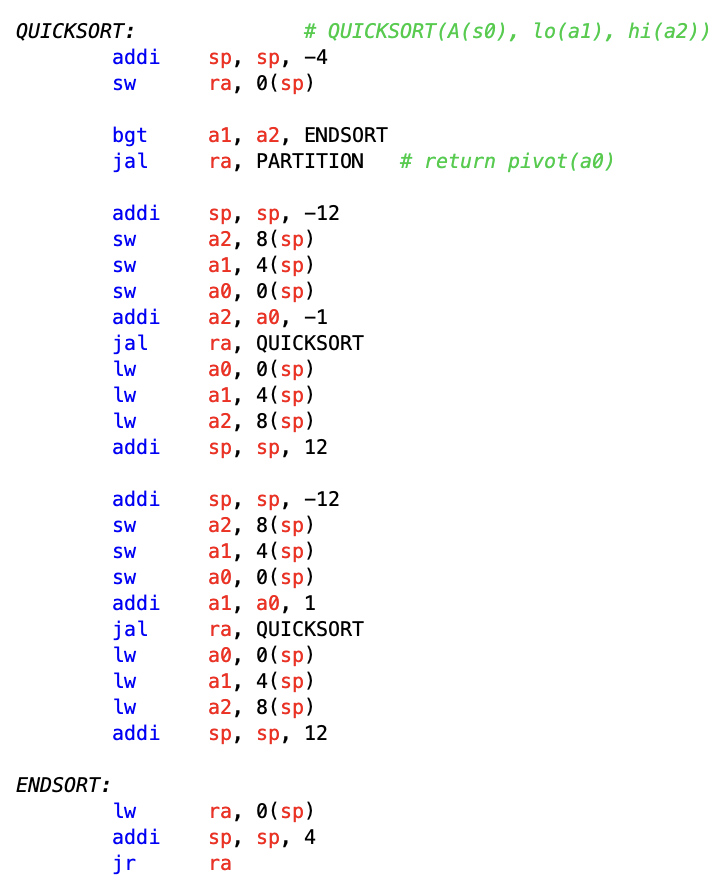
\includegraphics[scale = 0.7]{Lab1-3-3.png}\\
					\hline
				\end{tabular}
		\end{center}
        
    \end{table}
	\begin{table}[htbp]
        \begin{center}
			\caption{Main Code for Question 3(continue)}
				\begin{tabular}[H]{|M{3cm}|M{12cm}|}
					\hline
					Function & Code\\

					\hline
					PARTITION
					& 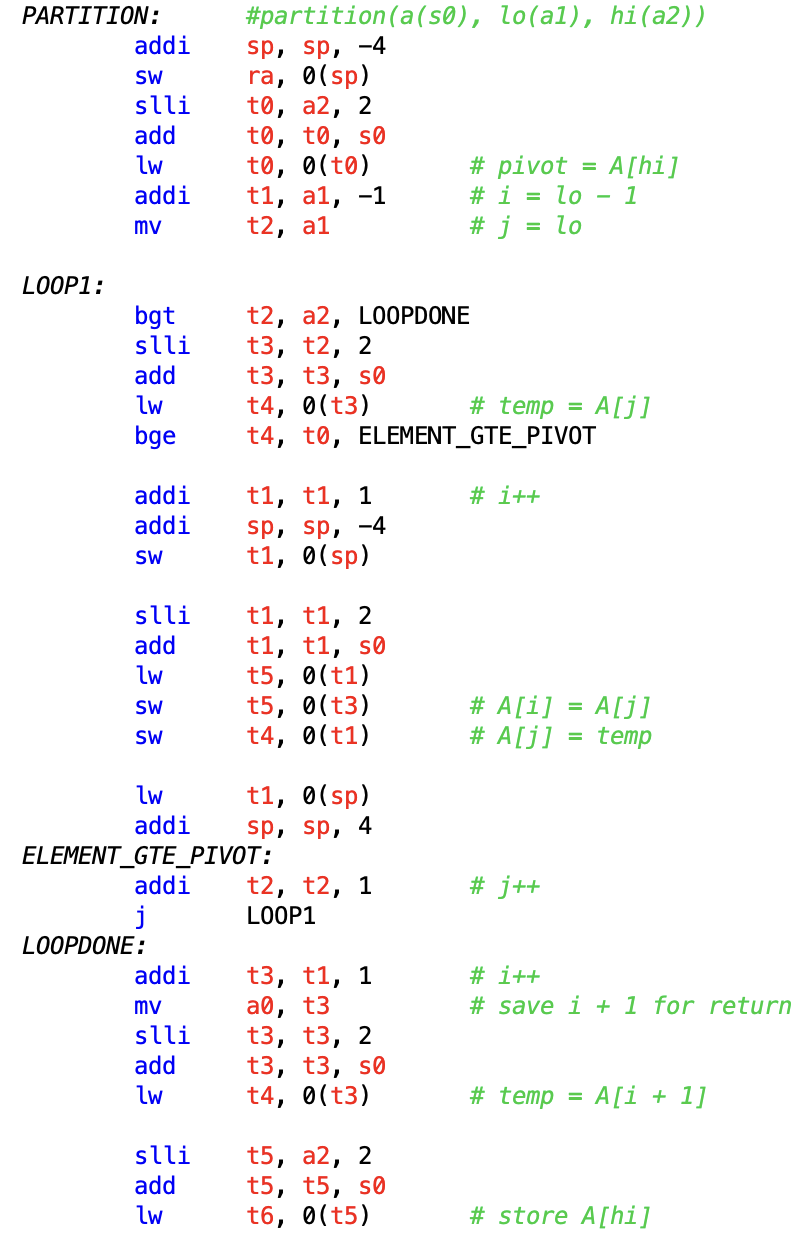
\includegraphics[scale = 0.8]{Lab1-3-4.png}\\

					\hline
				\end{tabular}
		\end{center} 
    \end{table}

	\begin{figure}[H]
		\caption{Console Results(Output: Last line)}
		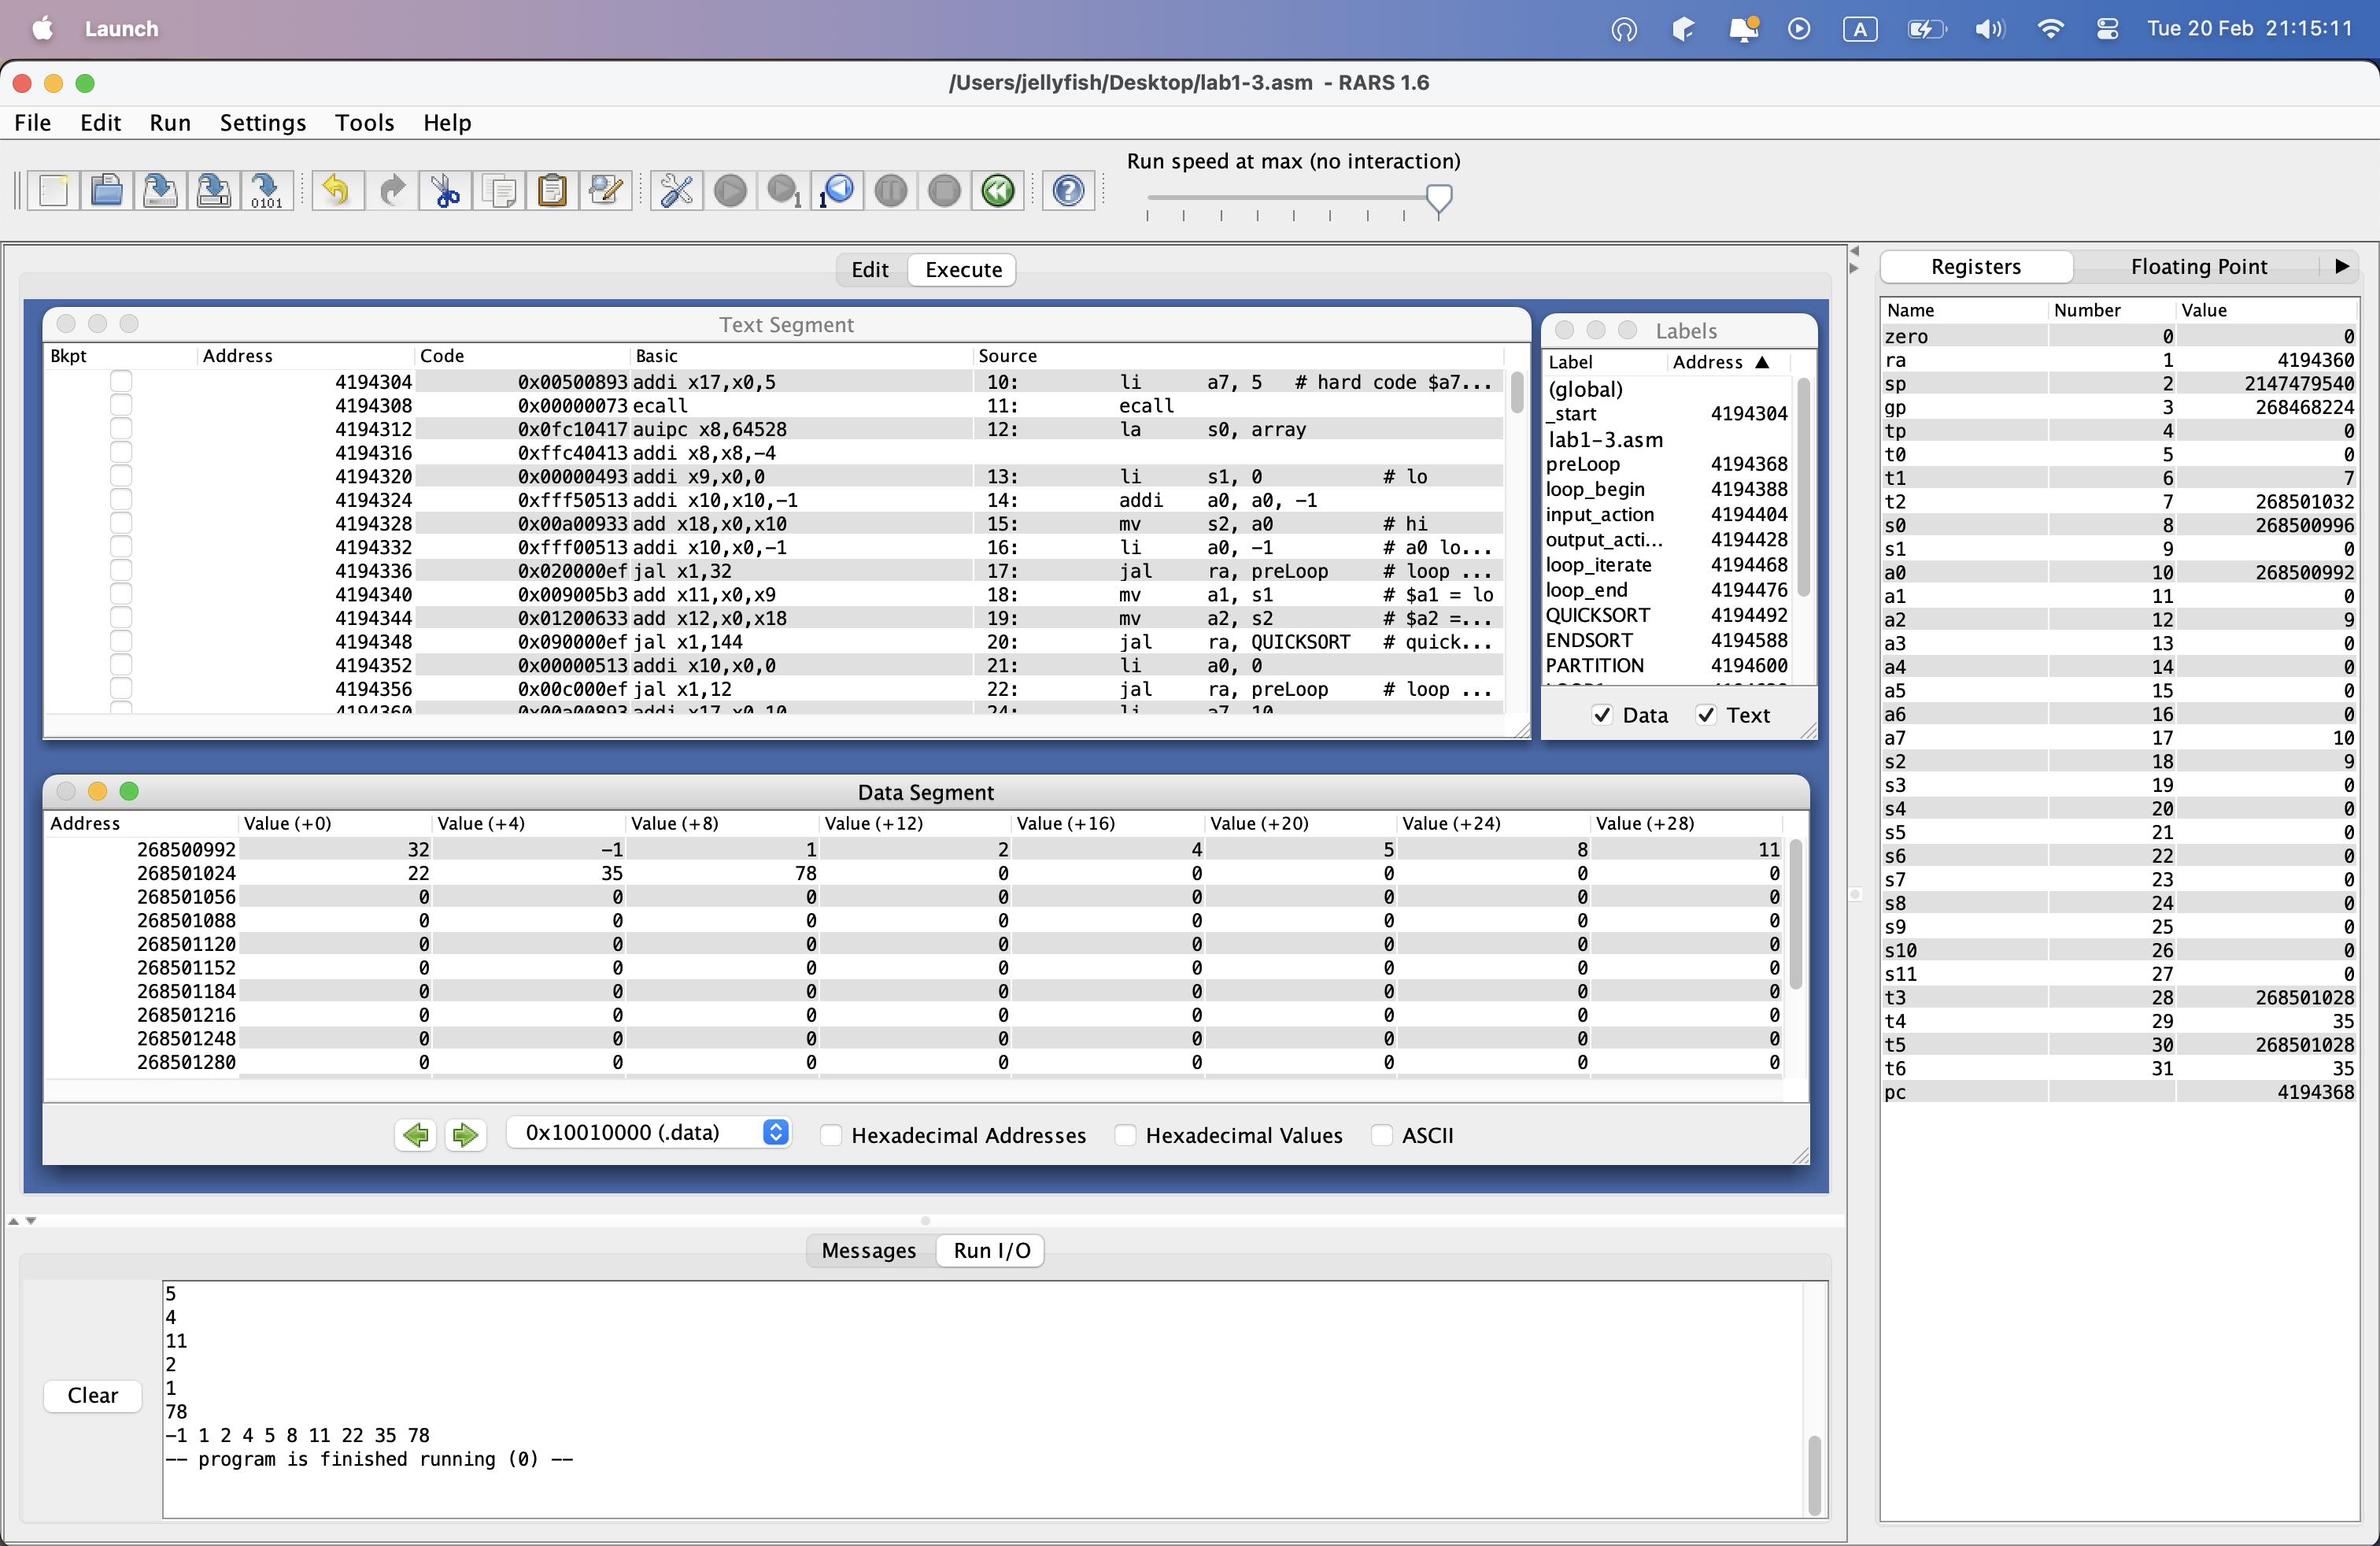
\includegraphics[width=1\linewidth]{Lab1-3-1.png}
	\end{figure}
\end{ans}
\end{document}